\documentclass{article}

\usepackage{biblatex}
\addbibresource{sources.bib}

\usepackage{csquotes}

\usepackage{graphicx}

\usepackage{multicol}

\title{Plan van aanpak - IPASS}
\author{Jimmy Bierenbroodspot}
\date{5 juni 2024}

\begin{document}
\begin{titlepage}
  \maketitle
\end{titlepage}

\section{Probleembeschrijving}

In de toekomst willen wij graag een AI-model hebben, dat de beste CV's op de
markt kan maken voor onze klanten. Hiervoor hebben we natuurlijk veel data in de
vorm van CV's nodig en gelukkig hebben we deze in grote aantallen. Nu is het
probleem dat deze CV's in .pdf-formaat opgeslagen zijn en text hieruit halen is
niet makkelijk \cite{timalsina-2024}.

We hebben het programma genaamd PyPDF\cite{unknown-author-2024} waarmee we in
staat zijn om text uit .pdf-bestanden te lezen, het probleem is dat dit
ongestructureerd is. Als voorbeeld kunnen we het voorbeeld CV in \ref{fig:cv-example}
nemen.

\begin{figure}[ht]
  \begin{center}
    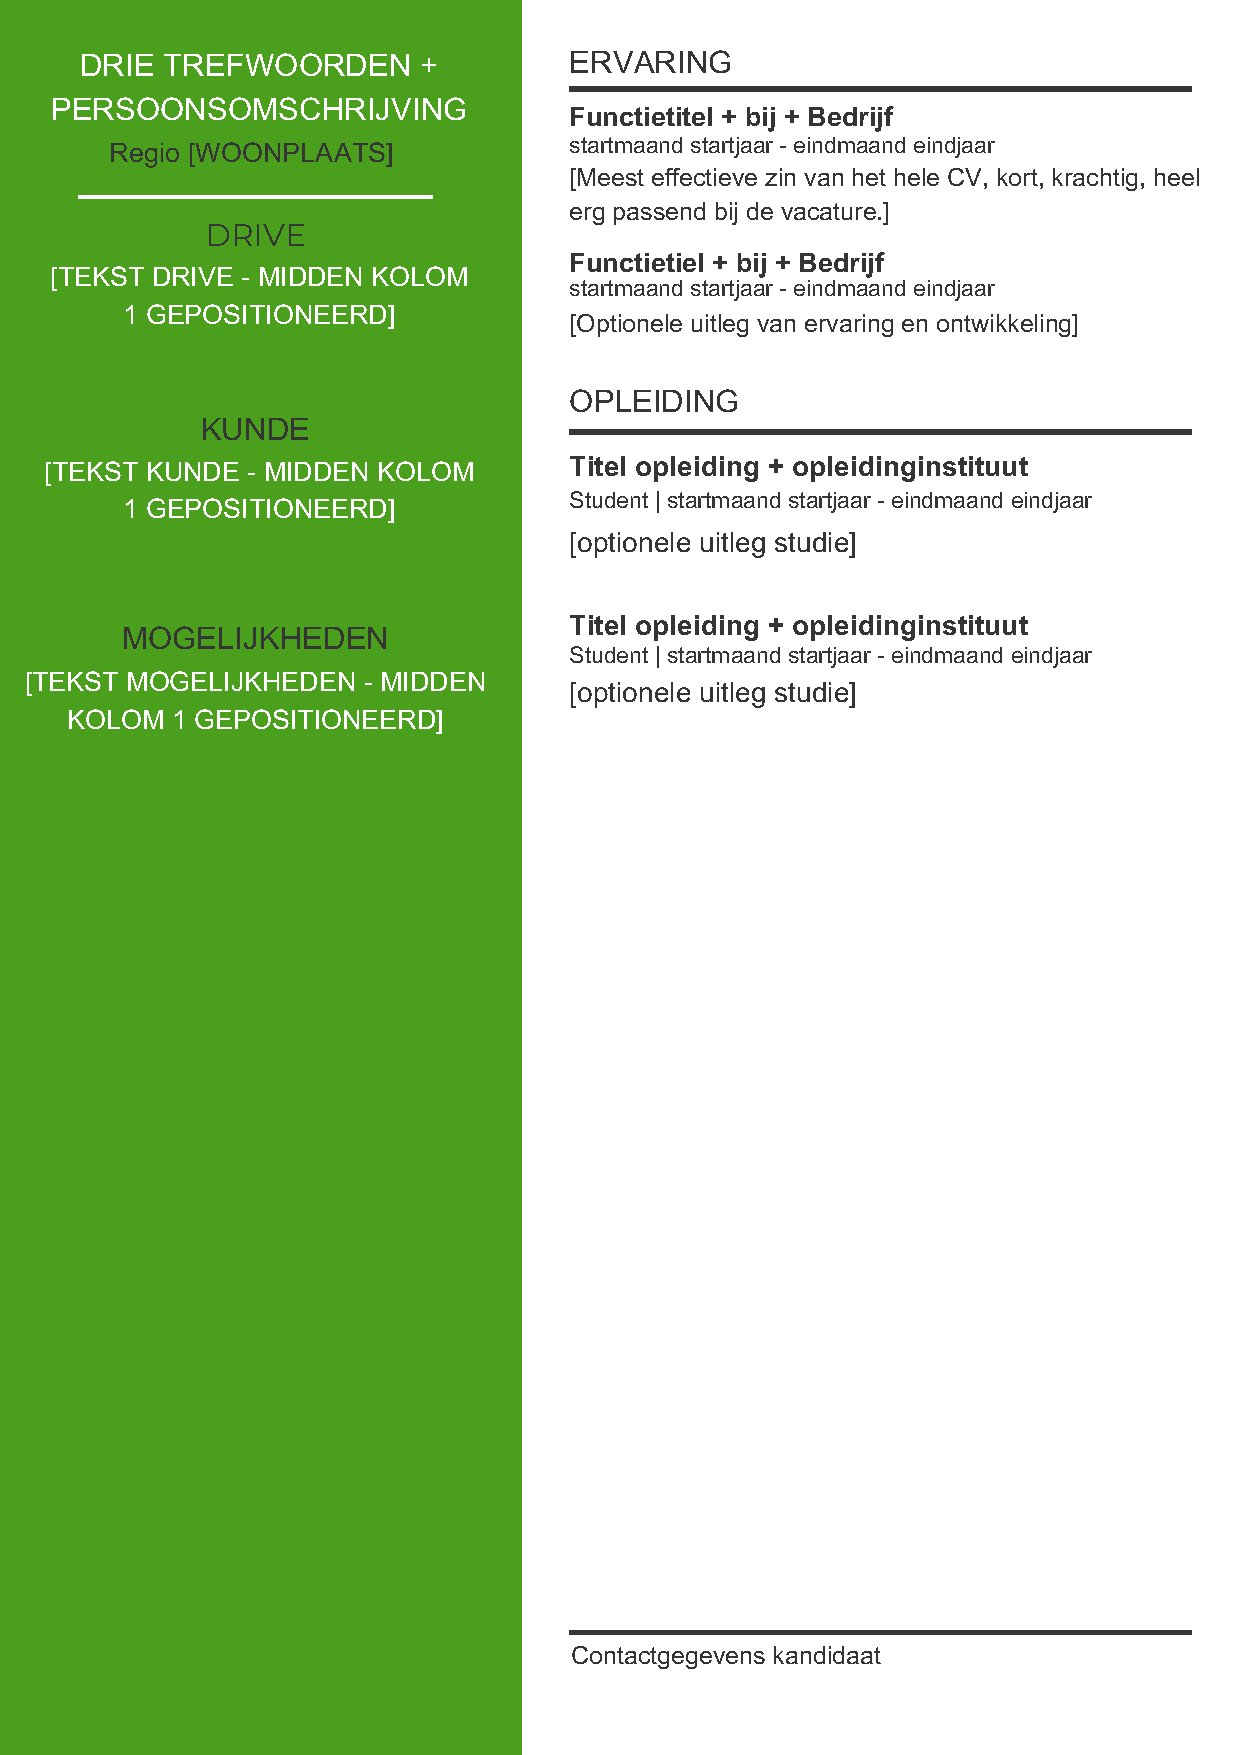
\includegraphics[width=0.5\linewidth]{pdf/voorbeeld_aicv_cv.pdf}
  \end{center}
  \caption{Voorbeeld van een Cliq CV}
  \label{fig:cv-example}
\end{figure}

In \ref{fig:pypdf-no-layout} kunnen we zien wat er gebeurd als we de tekst
uit \ref{fig:cv-example} lezen. Dit ziet er uit als een onlogisch rommeltje.
We kunnen met PyPDF echter ook de tekstopmaak kopiëren, zoals te zien in
\ref{fig:pypdf-w-layout}. Dit ziet er al beter uit maar als we bedenken dat
dit allemaal op een regel staat, waarbij de nieuwe regels in dit geval juist
worden getoond, maar eigenlijk aangeduid wordt met een \textbackslash n.

\begin{figure}[ht]
  \begin{center}
    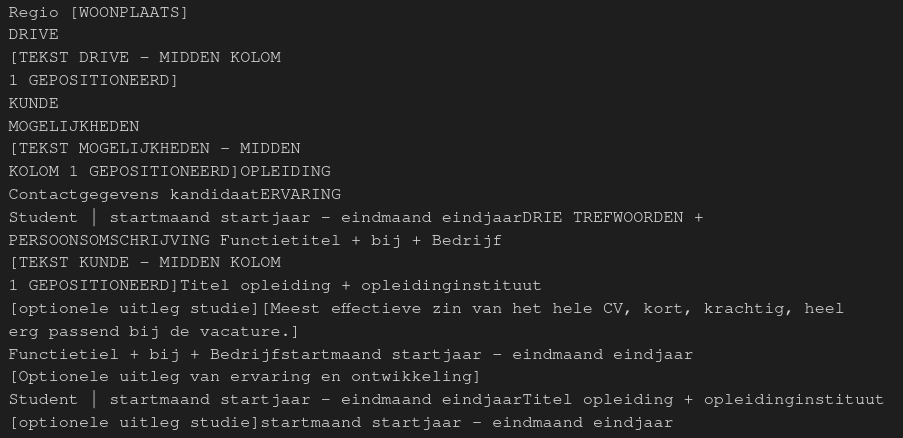
\includegraphics[width=\linewidth]{img/voorbeeld_pypdf_text_extract_geen_layout.png}
  \end{center}
  \caption{Voorbeeld van tekstextractie PyPDF}
  \label{fig:pypdf-no-layout}
\end{figure}

\begin{figure}[ht]
  \begin{center}
    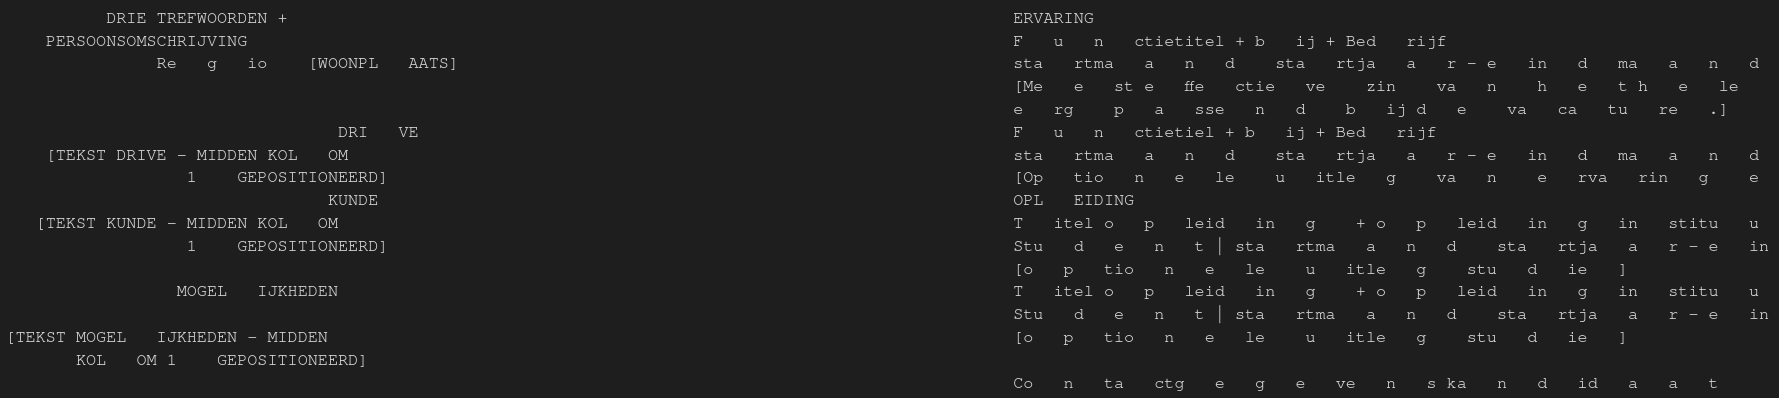
\includegraphics[width=\linewidth]{img/voorbeeld_pypdf_text_extract_layout.png}
  \end{center}
  \caption{Voorbeeld van tekstextractie PyPDF met tekstopmaak}
  \label{fig:pypdf-w-layout}
\end{figure}

\vfill

\subsection{Waarom willen we dit?}

In datawetenschap kennen we het concept GIGO, oftewel garbage in garbage out
\cite{merriam-webster-no-date}. Als we aannemen dat ditzelfde zal gelden voor
het model dat we gaan gebruiken dan zouden we graag willen dat onze invoerdata
gestructureerd is.

Als we aannemen dat de tekst op een regel zou moeten komen te staan om ingelezen
te worden door het model, dan zijn beide manieren van text extraheren met PyPDF
niet gestructureerd. We willen dus dat de tekst op een logische volgorde komt te
staan. Als een CV geen kolommen zou bevatten dan kunnen we met PyPDF de
tekstopmaak kopiëren, nu weten we alleen van tevoren niet of een CV kolommen
heeft of niet en als dat wel zo is weten we niet hoeveel kolommen er zijn. Om
hierachter te komen moeten we naar het CV kijken en dat gaat niet met een
geautomatiseerd proces.

\section{Algoritme}

In \ref{fig:pypdf-w-layout} kunnen we zien dat er een best duidelijke scheiding
zit tussen de twee kolommen. Als we aannemen dat dit het geval is voor elke CV
dan kunnen we een heuristiek opzetten om te bepalen hoeveel kolommen zich in een
document bevinden. Vervolgens kunnen we deze informatie gebruiken om alle tekst
op chronologische leesvolgorde onder elkaar te zetten.

\subsection{Heuristiek}

We kunnen de stappen voor de heuristiek als volgt op een rij zetten:

\begin{enumerate}
  \item Haal de tekst uit het document d.m.v. PyPDF.
  \item Vind de positie van de scheiding van de kolommen.
  \item Plaats de kolommen onder elkaar met gebruik van de kolomscheiding.
\end{enumerate}

Nu is het wat lastiger om erachter te komen waar de scheiding tussen de kolommen
precies zitten. Hier komt het algoritme van pas.

\subsection{Welk algoritme?}

Wat we hier proberen te doen staat bekend als "page/document layout analysis",
een techniek om de opmaak van een pagina te bepalen \cite{o-gorman-1993}.
Omdat we in het huidige stadium alleen gebruik maken van bestaande LLM's,
hoeven we geen algoritme te gebruiken om te begrijpen wat elk stukje tekst
betekent. Het enige dat er voor nu echt toe doet is dat de tekst in een logische
en chronologische volgorde staat. Ook willen we ons nog niet gaan focussen op
CV's met een complexe opmaak.

Omdat we de tekstopmaak al in tekstvorm hebben (zie \ref{fig:pypdf-w-layout})
lijkt het mogelijk om een relatief simpel clusteringsalgoritme, zoals Llyods
algoritme \cite{lloyd-1982}, te gebruiken om samen met de elleboog methode om de
kolommen in het document te vinden.

\section{Taken}

Voor dit project zijn de volgende taken benodigd:

\subsection{Applicatie}

\begin{enumerate}
  \item Simpele UI d.m.v. Jupyter Notebook | Noodzakelijk | 2 u.
  \item Een UI d.m.v. een front-end framework | Optioneel | 6 u.
\end{enumerate}

\subsection{Algoritme}

\begin{enumerate}
  \item Verkrijgen van tekst uit pdf-bestanden | Noodzakelijk | 1 u.
  \item Implementeren van algoritme volgens bron | Noodzakelijk | 6 u.
  \item Andere/betere algoritme implementeren | Optioneel | 6 u.
\end{enumerate}

\subsection{Rapportage}

\begin{enumerate}
  \item Probleembeschrijving | Noodzakelijk | 1 u.
  \item Beschrijving van eisen | Noodzakelijk | 1 u.
  \item Beschrijving van algoritme | Noodzakelijk | 1 u.
  \item Evalueren van algoritme | Optioneel | 4 u.
  \item Poster | Noodzakelijk | 6 u.
\end{enumerate}

\section{Planning}

\begin{table}[ht]
  \centering
  \begin{tabular}{|l|l|}
    \hline
    \textbf{Week} & \textbf{Taken}                           \\
    \hline
    23            & - Implementeren van algoritme beginnen   \\
                  & - Verkrijgen van tekst uit pdf-bestanden \\
                  & - Simpele UI d.m.v. Jupyter Notebook     \\
    \hline
    24            & - Implementeren afmaken                  \\
                  & - Zoeken naar andere algoritme           \\
                  & - Evalueren van algoritme                \\
    \hline
    25            & - Betere UI                              \\
                  & - Rapport: Probleembeschrijving          \\
                  & - Rapport: Beschrijving van eisen        \\
                  & - Rapport: Beschrijving van algoritme    \\
    \hline
    26            & - Poster                                 \\
                  & - Uitloop                                \\
    \hline
  \end{tabular}
  \caption{De planning}
  \label{tab:planning}
\end{table}

\section{Risico's}

\subsection{Risico: afwijking van scope}

Het is een risico dat er afgeweken kan worden van de originele scope en voorzie
dat de kans dat dit gebeurt groot is. Dit betekent dat het mogelijk is dat er
naar dingen gekeken gaan worden die niet leiden naar het verwachte resultaat. De
impact hiervan zou groot zijn aangezien dit kan leiden tot een incompleet
product of missende onderdelen.

Dit kan vermeden worden door een duidelijk beeld te hebben van wat er gedaan
moet worden en door en docenten op polshoogte te houden.

\subsection{Risico: Incorrect ontwikkelen van het algoritme}

Er is een risico dat het algoritme incorrect ontwikkeld kan worden en ik voorzie
dat de kans hiervan gemiddeld is. De impact hiervan is groot.

Dit kan vermeden worden door een goed besef te hebben van de bron, pseudocode te
gebruiken en tests voor de code te schrijven.

\subsection{Risico: Inefficient algoritme}

Er is een risico dat het algoritme Inefficient is, de kans dat dit gebeurt zal
groot zijn. De impact hiervan is relatief klein aangezien er niet met al te veel
data gewerkt hoeft te worden in de casus.

Dit kan vermeden worden door efficiënte datastructuren te gebruiken en zo min
mogelijk code te schrijven.

\printbibliography

\listoffigures

\listoftables

\end{document}